\section{Design and construction}\label{sec:design}
\sectionstate{partial}{\texttt{docs/detector\_spec/spec.py} (97 numbers, 9 unknown, 31 assumed);
spec page \texttt{notes/mx17-detector-spec.html}; Gerber files. v2 2026-11-10: the design choices are stated here
without their results (those are in \cref{sec:conclusions}); the parts list of the old figure caption is now
\cref{tab:layers}; the material in front of the drift volume is new (\cref{tab:material}).}
\intent{A complete, citable description of the chamber, layer by layer, and of how it was built and
qualified. Most of this section is Stephan's: the production side is not in our analysis repository.}

\subsection{Design choices}\label{sec:design_choices}
\askStephan{Dylan (2026-11-02): the section is yours to write; these are the design points we think a reader needs. What
the data say about each has moved to the conclusions (\cref{sec:conclusions}), so that results are not quoted before the
detector and the setups are described. Keep, reword or drop as you see fit.}
Four choices set these chambers apart from a standard bulk Micromegas.

\textbf{(1) Pads for an equal X/Y charge share.} The readout is a single plane of square pads, each routed to an X
or a Y strip, instead of two stacked strip layers, so that both views see the same charge
(\crefp{fig:chamber}{c}). The cost is one more copper layer in the board.

\textbf{(2) A resistive Micromegas in TPC mode.} The resistive layer protects the chamber against discharges, which a
pulsed, high-intensity facility makes likely: on the bench a discharge costs no measurable dead time
(\cref{app:discharges}). It also spreads the charge of each avalanche along the resistive strips. In a TPC that adds, in
one view, to the mixing of charge from different drift depths onto each strip that diffusion and the footprint of the
avalanche already cause, and so to the bias of per-strip hit times~\cite{paperIIb}. Once the waveforms are fitted with
a model of the charge spreading (\cref{sec:reco}) it costs little: the view read along the resistive strips is not
systematically worse than the other (\cref{sec:tracking}).

\textbf{(3) Resistive strips rather than a uniform resistive layer.} A continuous resistive layer was tried
first: it came out with too low a resistance, and current flowed through ``hot spots''. Resistive strips with the
strip ends passivated allowed a higher resistance and far less current. \emph{Stephan: the measured resistances and
currents of the uniform-layer boards, if they exist.}

\textbf{(4) Strip direction and passivation.} The strips run along $y$ and end at the two $y$ edges, where their
terminations are passivated (covered) over 18.0 and 18.7\,mm (\crefp{fig:chamber}{b}). \emph{Stephan: why the
passivation is needed (the termination / HV connection at the strip ends, and discharges there?).} This removes about
10\,\% of the area. The orientation was chosen mainly for where that loss falls: at the top and bottom of the chamber,
not on the sides that face the neighbouring chambers at n\_TOF. Better resolution was also expected across the strips
than along them, since the charge spreads along them. The two $x$ sides are not passivated.

\subsection{Chamber layout}
\tbw{Entrance window and flange, 30\,mm drift gap, cathode, field cage. Active area.}
\askStephan{Field cage: number of ring strips per board, pitch and width, resistor chain. Was chamber B's field cage missing or damaged?}
\askStephan{Window: 60\,\textmu m mylar? aluminised on one side or both, Al thickness, which side faces the gas.
Cathode: 50\,\textmu m kapton with copper on one side, copper thickness. Operating overpressure / window bulge;
is the drift gap exactly 30.0\,mm at the centre under pressure? (We measure 28.2\,mm on chamber~A, \cref{sec:gap}.)}
The pads cover $399.4\times399.4$\,mm$^2$ ($512\times0.78$\,mm). There is no passivation in $x$; in $y$ the ends of
the resistive strips are passivated over about 19\,mm on each side (17.9 to 20.4\,mm over the five chambers; 18.0 and
18.7\,mm on chamber~A), which leaves an efficient length of $359.9\pm1.8$\,mm.
\askDylan{Rundown item 3: $359.9\pm1.8$\,mm is the mean of seven measurements over several chambers (bench and beam), not
chamber~A's value (361.9\,mm from its own 50\,\% points on the bench, 357.2\,mm in the beam). Strip coordinates run from 0 to
398.6\,mm (the start of the last strip); 399.4\,mm is the width. The old text subtracted A's bands from the width.}

\begin{table}[tbp]
  \centering\small
  \caption{Layers of a chamber at the centre of the active area, from the target side (\cref{fig:chamber}).
  $^\dagger$: assumed or not yet confirmed.}
  \label{tab:layers}
  \begin{tabular}{lll}
    \hline
    layer & material and pattern & thickness \\
    \hline
    entrance window & Mylar & 60\,\textmu m \\
    gas gap & chamber gas & 5.0\,mm \\
    drift cathode, at $-HV_\mathrm{drift}$ & Kapton with copper$^\dagger$ & 50\,\textmu m, 9\,\textmu m$^\dagger$ \\
    drift gap & chamber gas & 30\,mm (design) \\
    mesh$^\dagger$, at ground & woven steel, 19\,\textmu m wire on a 67\,\textmu m pitch & \\
    amplification gap & gas; pillars \O\,0.6\,mm on a 4.68\,mm grid & 150\,\textmu m \\
    resistive strips$^\dagger$, at $+HV_\mathrm{resist}$ & 550\,\textmu m wide on a 0.80\,mm pitch, along $y$ & 10\,\textmu m \\
    insulator$^\dagger$ & Kapton and glue & 70.5\,\textmu m \\
    pads & copper, 0.68\,mm on a 0.78\,mm pitch & 26\,\textmu m$^\dagger$ \\
    Y strips, X strips & copper, each joined by vias to every second pad & \\
    readout board & FR4$^\dagger$, 264\,\textmu m per layer & 1.70\,mm \\
    Rohacell & & 5\,mm \\
    back foil & Mylar & 25\,\textmu m$^\dagger$ \\
    support plate & aluminium, open over a 402\,mm aperture & 8\,mm \\
    \hline
  \end{tabular}
\end{table}

\subsection{Material in front of the measurement}\label{sec:material}
\sectionstate{partial}{new 2026-11-10; \texttt{papers/paper1\_v2/figs/out/material\_budget.json} (Highland, thicknesses of \cref{tab:layers}).
The cathode copper thickness is assumed: Stephan to confirm, it is the largest entry.}
The chambers are meant as low-material trackers, so the material a lepton crosses before and while it is measured is
part of the design. \Cref{tab:material} lists it with the multiple scattering it causes.
% Numbers: figs/out/material_budget.json (figs/make_material_budget.py). Highland, per projection, electron momentum.
\begin{table}[tbp]
  \centering\small
  \caption{Material between the target and the end of the drift gap at normal incidence, and the multiple scattering
  it causes: rms angle $\theta_0$ per projection for electrons of 4, 8 and 16\,MeV kinetic energy (Highland formula;
  the summed rows apply it to the summed thickness). The aluminisation of the window is ignored. $^\dagger$: the copper
  thickness of the cathode is assumed.}
  \label{tab:material}
  \begin{tabular}{llrrrr}
    \hline
     & & & \multicolumn{3}{c}{$\theta_0$ [\textdegree] at} \\
    layer & thickness & $x/X_0$ [\%] & 4\,MeV & 8\,MeV & 16\,MeV \\
    \hline
    air, target to window & 200\,mm & 0.066 & 3.24 & 1.70 & 0.88 \\
    entrance window, Mylar & 60\,\textmu m & 0.021 & 1.72 & 0.90 & 0.47 \\
    gas gap & 5\,mm & 0.004 & 0.70 & 0.37 & 0.19 \\
    drift cathode, Kapton & 50\,\textmu m & 0.018 & 1.55 & 0.82 & 0.42 \\
    drift cathode, copper$^\dagger$ & 9\,\textmu m & 0.063 & 3.16 & 1.66 & 0.85 \\
    \hline
    in front of the drift volume & & 0.171 & 5.49 & 2.88 & 1.48 \\
    \quad without the copper$^\dagger$ & & 0.109 & 4.27 & 2.24 & 1.15 \\
    \hline
    drift gas, Ar/iC$_4$H$_{10}$ 95/5 & 28.2\,mm & 0.024 & 1.83 & 0.96 & 0.49 \\
    \hline
  \end{tabular}
\end{table}


\subsection{Amplification stage and resistive layer}
\tbw{Bulk Micromegas: mesh, amplification gap, pillars. Resistive strips over the pads, insulator, how the charge
reaches the pads (capacitive coupling through the insulator).}
\askStephan{Mesh: material, wire diameter, opening, thickness, supplier; calendered, and its thickness after?
Amplification gap 150\,\textmu m? photoresist and number of laminations; pillars \O\,0.6\,mm on a 4.68\,mm grid?}
\askStephan{Resistive strips: width and pitch (550/800\,\textmu m, while the readout pitch is 780\,\textmu m?), direction,
number; thickness after curing; paste grade and supplier; sheet resistance or end-to-end resistance (any measurement on these boards?);
the insulator between strips and pads (kapton thickness, adhesive type and thickness).}

\subsection{Readout board}
\tbw{512\,$\times$\,512 square pads (0.68\,mm on a 0.78\,mm pitch), each connected by a via to an X strip or a
Y strip. Connectors, DREAM front-end, channel count.}
\askStephan{Confirm the readout scheme and which pads go to which view. Is there a stack-up drawing
(layer order, copper and dielectric thicknesses)? Behind the board: Rohacell grade and the back mylar.}
\askStephan{We measure a $\sim$19\,mm dead band at each end of Y on every chamber. Is that the covered copper bus
where the resistive strips are terminated?}

\begin{figure}[tbp]
  \centering
  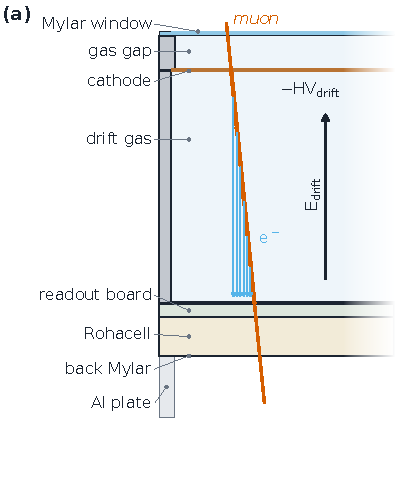
\includegraphics{chamber_stack_a}\hfill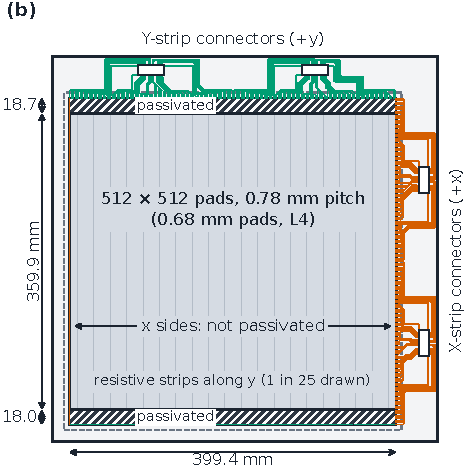
\includegraphics{readout_layout_b}\\[6pt]
  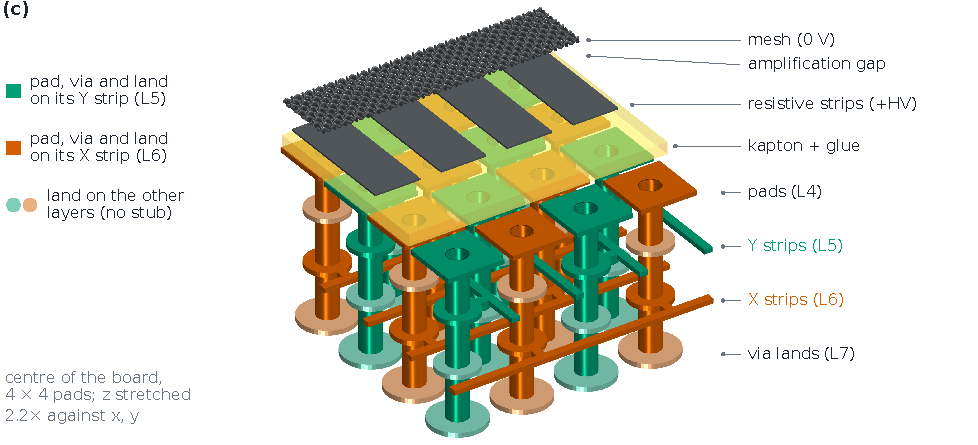
\includegraphics{readout_stack_3d}
  \caption{A chamber. (a) Cross-section through the centre of the active area, $z$ to scale and $x$ cut off on the right
  (the chamber is 440\,mm wide): window, gas gap, drift cathode, the drift gap with an inclined muon whose ionisation
  electrons drift to the mesh, the readout board, Rohacell, back foil and the aluminium plate. (b) The readout board
  from above, from the production Gerber files: $512\times512$ pads, the Y strips running along $y$ to two connectors on
  the $+y$ edge and the X strips along $x$ to two connectors on the $+x$ edge; the resistive strips run along $y$ (faint
  lines, one in 25 drawn) and are passivated at their ends (hatched). (c) Four by four pads at the centre of the board,
  from the mesh down to L7, drawn in 3D from the same Gerber files with $z$ stretched 2.2 times against $x$ and $y$:
  mesh, amplification gap (33\,kV/cm at 490\,V), resistive strips, kapton, pads, and the Y and X strips. Each layer
  above the pads starts one pad row further back, and the FR4 between the copper layers is not drawn. Every pad has one
  plated via, drilled from the pad layer to L7, with a copper land on each layer it crosses; a land joins a strip, by a
  short stub, only on that strip's own layer. Pads alternate between the two views in a checkerboard, so every strip
  collects every second pad along its length; pad, via and joined land take the colour of their strip, and the lands
  without a stub are drawn light. L4, L5 and L6 are the copper layers of the board that carry the pads, the Y strips
  and the X strips; under the active area L7 carries only the lands at the foot of the vias. The weave of the mesh and
  the position of the resistive strips against the pads are schematic. Dimensions: \cref{tab:layers}.}
  \label{fig:chamber}
\end{figure}

\subsection{Production and quality control}
\tbw{How many boards were built, where and when; the bulk process; the resistive-layer printing; acceptance tests
(resistance mapping, HV training, leak and gas tightness, gain uniformity). Which board went into which chamber.}
\askStephan{This subsection is yours: production sequence, QA steps and their results, and anything that
distinguishes the boards of chambers A--E (in particular chamber~E's board, \cref{app:beam}).}
